\documentclass{standalone}
\usepackage{tikz}
\usepackage{xcolor}
\usetikzlibrary{patterns, positioning}

    \usetikzlibrary{calc}
    \usepackage{relsize}
    \tikzset{fontscale/.style = {font=\relsize{#1}}}
\begin{document}
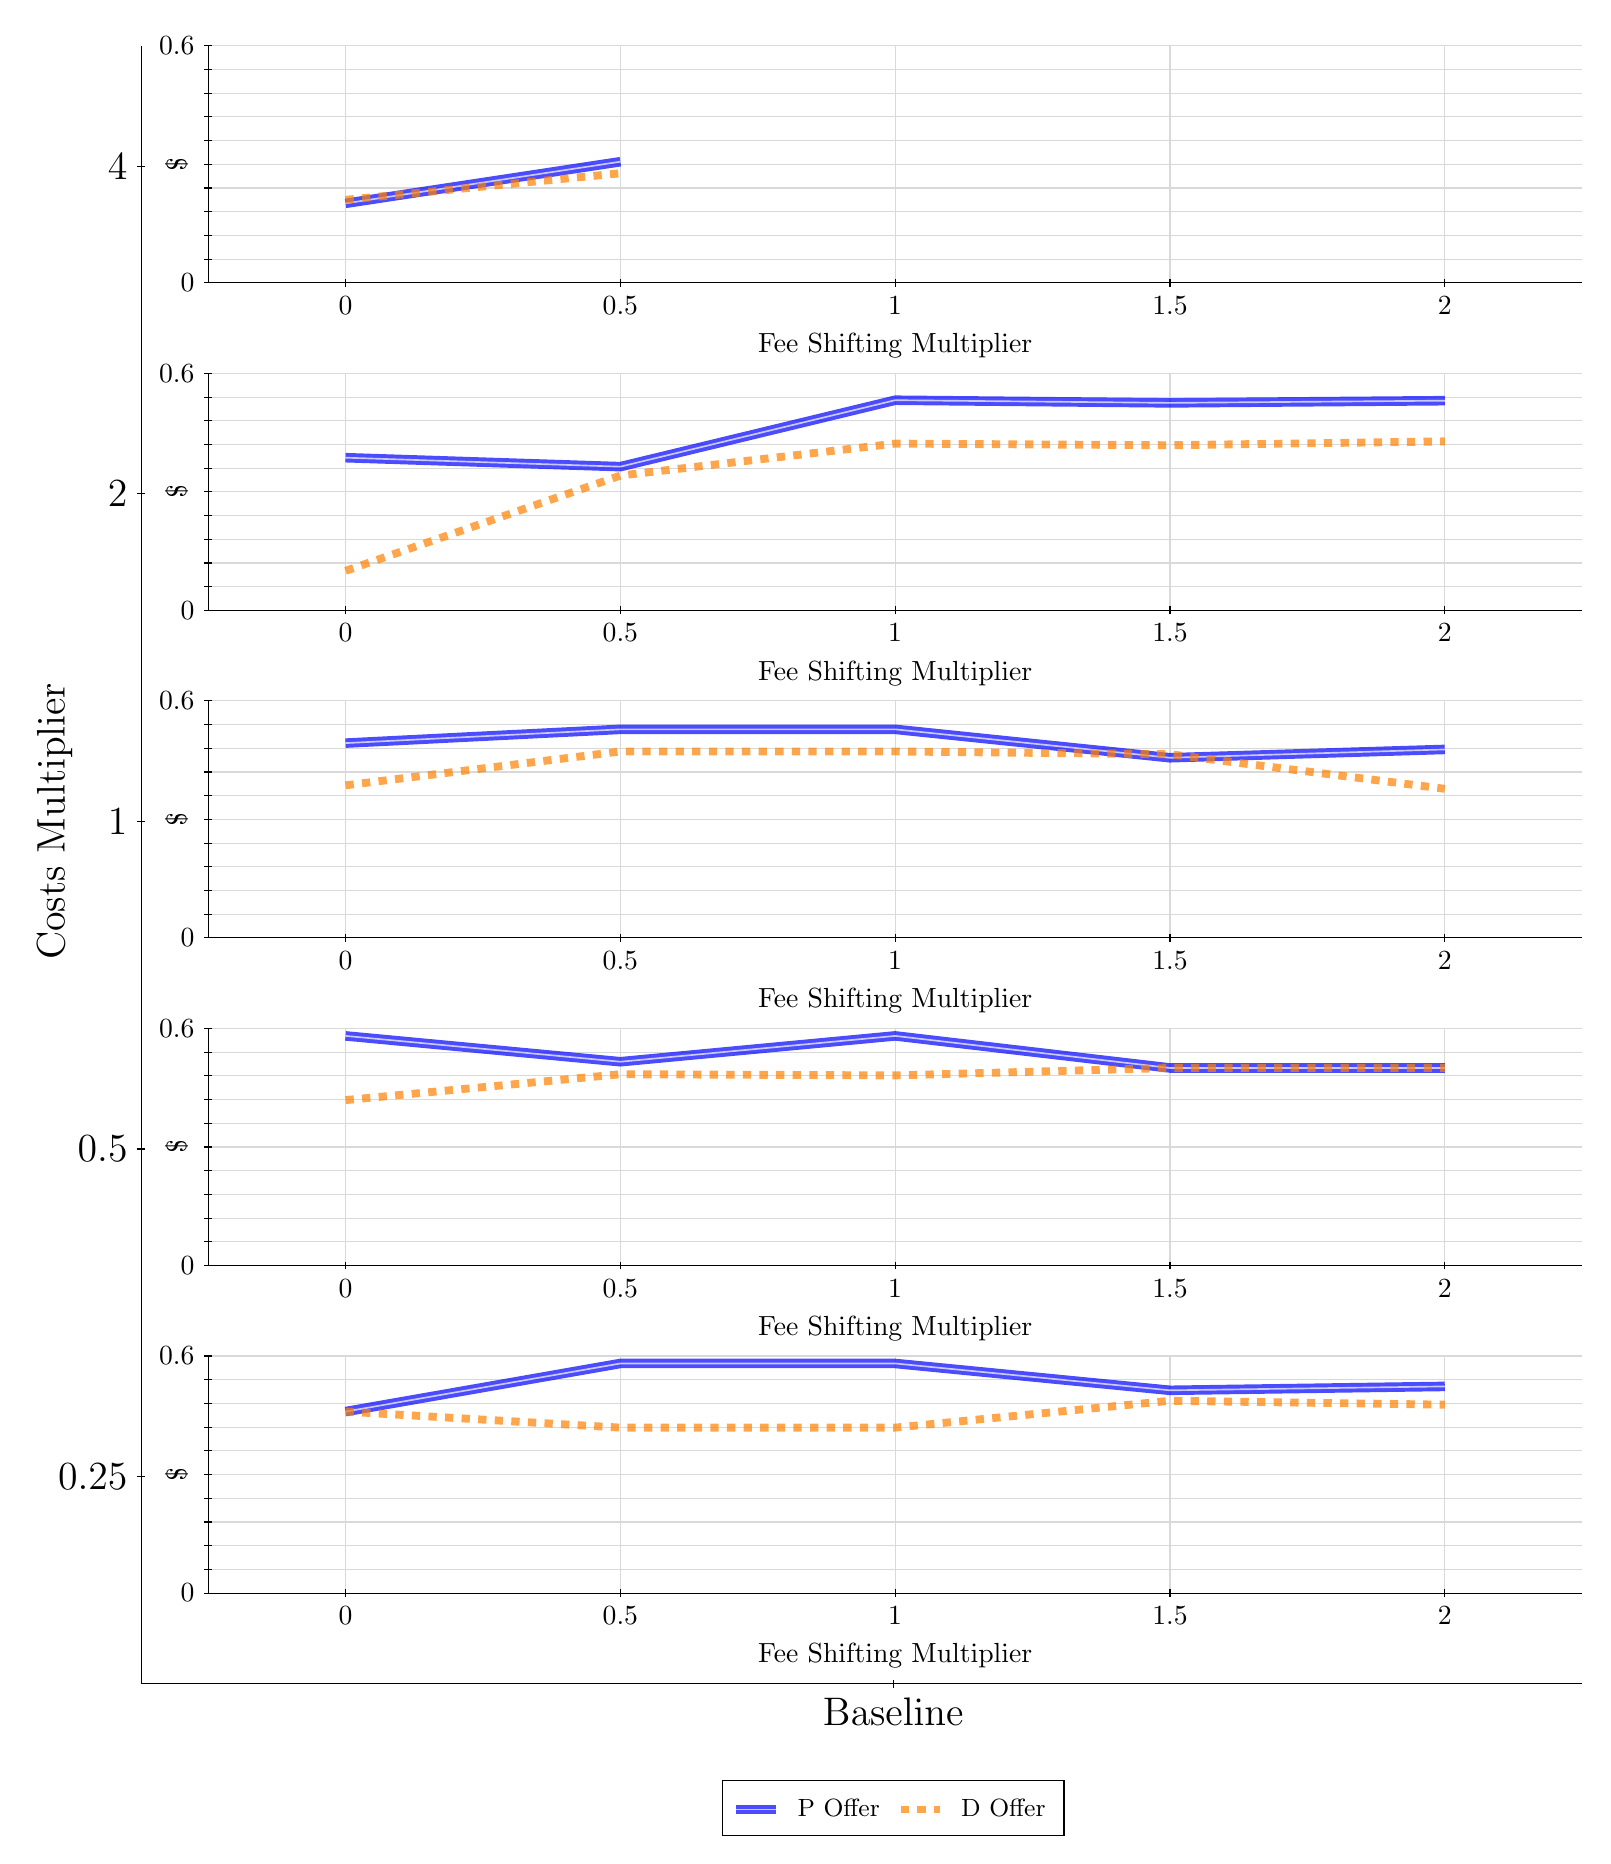
\begin{tikzpicture}
\draw[black] (1.7,1.5) -- (1.7,22.3);
\node[rotate=90, fontscale=2, anchor=center] at (0.6, 12.45) {Costs Multiplier};
\draw[black] (1.65,4.13) -- (1.75,4.13);
\node[fontscale=2, anchor=east] at (1.65, 4.13) {0.25};
\draw[black] (1.65,8.29) -- (1.75,8.29);
\node[fontscale=2, anchor=east] at (1.65, 8.29) {0.5};
\draw[black] (1.65,12.45) -- (1.75,12.45);
\node[fontscale=2, anchor=east] at (1.65, 12.45) {1};
\draw[black] (1.65,16.61) -- (1.75,16.61);
\node[fontscale=2, anchor=east] at (1.65, 16.61) {2};
\draw[black] (1.65,20.77) -- (1.75,20.77);
\node[fontscale=2, anchor=east] at (1.65, 20.77) {4};

\draw[black] (1.7,1.5) -- (20,1.5);
\node[fontscale=2, anchor=center] at (11.25, 0.6) {};
\draw[black] (11.25,1.45) -- (11.25,1.55);
\node[fontscale=2, anchor=north] at (11.25, 1.45) {Baseline};


\draw[gray!30] (2.55,2.65) -- (20,2.65);
\draw[gray!30] (2.55,2.951) -- (20,2.951);
\draw[gray!30] (2.55,3.252) -- (20,3.252);
\draw[gray!30] (2.55,3.553) -- (20,3.553);
\draw[gray!30] (2.55,3.854) -- (20,3.854);
\draw[gray!30] (2.55,4.155) -- (20,4.155);
\draw[gray!30] (2.55,4.456) -- (20,4.456);
\draw[gray!30] (2.55,4.757) -- (20,4.757);
\draw[gray!30] (2.55,5.058) -- (20,5.058);
\draw[gray!30] (2.55,5.359) -- (20,5.359);
\draw[gray!30] (2.55,5.66) -- (20,5.66);
\draw[gray!30] (4.295,2.65) -- (4.295,5.66);
\draw[gray!30] (7.785,2.65) -- (7.785,5.66);
\draw[gray!30] (11.275,2.65) -- (11.275,5.66);
\draw[gray!30] (14.765,2.65) -- (14.765,5.66);
\draw[gray!30] (18.255,2.65) -- (18.255,5.66);
\draw[black] (2.55,2.65) -- (2.55,5.66);
\node[rotate=90, fontscale=0.7, anchor=center] at (2.15, 4.155) {\$};
\draw[black] (2.5,2.65) -- (2.6,2.65);
\node[fontscale=0.7, anchor=east] at (2.5, 2.65) {0};
\draw[black] (2.5,2.951) -- (2.6,2.951);
\node[fontscale=0.7, anchor=east] at (2.5, 2.951) { };
\draw[black] (2.5,3.252) -- (2.6,3.252);
\node[fontscale=0.7, anchor=east] at (2.5, 3.252) { };
\draw[black] (2.5,3.553) -- (2.6,3.553);
\node[fontscale=0.7, anchor=east] at (2.5, 3.553) { };
\draw[black] (2.5,3.854) -- (2.6,3.854);
\node[fontscale=0.7, anchor=east] at (2.5, 3.854) { };
\draw[black] (2.5,4.155) -- (2.6,4.155);
\node[fontscale=0.7, anchor=east] at (2.5, 4.155) { };
\draw[black] (2.5,4.456) -- (2.6,4.456);
\node[fontscale=0.7, anchor=east] at (2.5, 4.456) { };
\draw[black] (2.5,4.757) -- (2.6,4.757);
\node[fontscale=0.7, anchor=east] at (2.5, 4.757) { };
\draw[black] (2.5,5.058) -- (2.6,5.058);
\node[fontscale=0.7, anchor=east] at (2.5, 5.058) { };
\draw[black] (2.5,5.359) -- (2.6,5.359);
\node[fontscale=0.7, anchor=east] at (2.5, 5.359) { };
\draw[black] (2.5,5.66) -- (2.6,5.66);
\node[fontscale=0.7, anchor=east] at (2.5, 5.66) {0.6};

\draw[black] (2.55,2.65) -- (20,2.65);
\node[fontscale=0.7, anchor=center] at (11.275, 1.85) {Fee Shifting Multiplier};
\draw[black] (4.295,2.6) -- (4.295,2.7);
\node[fontscale=0.7, anchor=north] at (4.295, 2.6) {0};
\draw[black] (7.785,2.6) -- (7.785,2.7);
\node[fontscale=0.7, anchor=north] at (7.785, 2.6) {0.5};
\draw[black] (11.275,2.6) -- (11.275,2.7);
\node[fontscale=0.7, anchor=north] at (11.275, 2.6) {1};
\draw[black] (14.765,2.6) -- (14.765,2.7);
\node[fontscale=0.7, anchor=north] at (14.765, 2.6) {1.5};
\draw[black] (18.255,2.6) -- (18.255,2.7);
\node[fontscale=0.7, anchor=north] at (18.255, 2.6) {2};

\draw[blue, opacity=0.70, line width=0.5mm, double] (4.295,4.9545) -- (7.785,5.5658) -- (11.275,5.5658) -- (14.765,5.2246) -- (18.255,5.2743);
\draw[orange, opacity=0.70, line width=1mm, dashed] (4.295,4.9545) -- (7.785,4.7508) -- (11.275,4.7508) -- (14.765,5.092) -- (18.255,5.0423);

\draw[gray!30] (2.55,6.81) -- (20,6.81);
\draw[gray!30] (2.55,7.111) -- (20,7.111);
\draw[gray!30] (2.55,7.412) -- (20,7.412);
\draw[gray!30] (2.55,7.713) -- (20,7.713);
\draw[gray!30] (2.55,8.014) -- (20,8.014);
\draw[gray!30] (2.55,8.315) -- (20,8.315);
\draw[gray!30] (2.55,8.616) -- (20,8.616);
\draw[gray!30] (2.55,8.917) -- (20,8.917);
\draw[gray!30] (2.55,9.218) -- (20,9.218);
\draw[gray!30] (2.55,9.519) -- (20,9.519);
\draw[gray!30] (2.55,9.82) -- (20,9.82);
\draw[gray!30] (4.295,6.81) -- (4.295,9.82);
\draw[gray!30] (7.785,6.81) -- (7.785,9.82);
\draw[gray!30] (11.275,6.81) -- (11.275,9.82);
\draw[gray!30] (14.765,6.81) -- (14.765,9.82);
\draw[gray!30] (18.255,6.81) -- (18.255,9.82);
\draw[black] (2.55,6.81) -- (2.55,9.82);
\node[rotate=90, fontscale=0.7, anchor=center] at (2.15, 8.315) {\$};
\draw[black] (2.5,6.81) -- (2.6,6.81);
\node[fontscale=0.7, anchor=east] at (2.5, 6.81) {0};
\draw[black] (2.5,7.111) -- (2.6,7.111);
\node[fontscale=0.7, anchor=east] at (2.5, 7.111) { };
\draw[black] (2.5,7.412) -- (2.6,7.412);
\node[fontscale=0.7, anchor=east] at (2.5, 7.412) { };
\draw[black] (2.5,7.713) -- (2.6,7.713);
\node[fontscale=0.7, anchor=east] at (2.5, 7.713) { };
\draw[black] (2.5,8.014) -- (2.6,8.014);
\node[fontscale=0.7, anchor=east] at (2.5, 8.014) { };
\draw[black] (2.5,8.315) -- (2.6,8.315);
\node[fontscale=0.7, anchor=east] at (2.5, 8.315) { };
\draw[black] (2.5,8.616) -- (2.6,8.616);
\node[fontscale=0.7, anchor=east] at (2.5, 8.616) { };
\draw[black] (2.5,8.917) -- (2.6,8.917);
\node[fontscale=0.7, anchor=east] at (2.5, 8.917) { };
\draw[black] (2.5,9.218) -- (2.6,9.218);
\node[fontscale=0.7, anchor=east] at (2.5, 9.218) { };
\draw[black] (2.5,9.519) -- (2.6,9.519);
\node[fontscale=0.7, anchor=east] at (2.5, 9.519) { };
\draw[black] (2.5,9.82) -- (2.6,9.82);
\node[fontscale=0.7, anchor=east] at (2.5, 9.82) {0.6};

\draw[black] (2.55,6.81) -- (20,6.81);
\node[fontscale=0.7, anchor=center] at (11.275, 6.01) {Fee Shifting Multiplier};
\draw[black] (4.295,6.76) -- (4.295,6.86);
\node[fontscale=0.7, anchor=north] at (4.295, 6.76) {0};
\draw[black] (7.785,6.76) -- (7.785,6.86);
\node[fontscale=0.7, anchor=north] at (7.785, 6.76) {0.5};
\draw[black] (11.275,6.76) -- (11.275,6.86);
\node[fontscale=0.7, anchor=north] at (11.275, 6.76) {1};
\draw[black] (14.765,6.76) -- (14.765,6.86);
\node[fontscale=0.7, anchor=north] at (14.765, 6.76) {1.5};
\draw[black] (18.255,6.76) -- (18.255,6.86);
\node[fontscale=0.7, anchor=north] at (18.255, 6.76) {2};

\draw[blue, opacity=0.70, line width=0.5mm, double] (4.295,9.7258) -- (7.785,9.3976) -- (11.275,9.7258) -- (14.765,9.3183) -- (18.255,9.3183);
\draw[orange, opacity=0.70, line width=1mm, dashed] (4.295,8.9108) -- (7.785,9.239) -- (11.275,9.2241) -- (14.765,9.3183) -- (18.255,9.3183);

\draw[gray!30] (2.55,10.97) -- (20,10.97);
\draw[gray!30] (2.55,11.271) -- (20,11.271);
\draw[gray!30] (2.55,11.572) -- (20,11.572);
\draw[gray!30] (2.55,11.873) -- (20,11.873);
\draw[gray!30] (2.55,12.174) -- (20,12.174);
\draw[gray!30] (2.55,12.475) -- (20,12.475);
\draw[gray!30] (2.55,12.776) -- (20,12.776);
\draw[gray!30] (2.55,13.077) -- (20,13.077);
\draw[gray!30] (2.55,13.378) -- (20,13.378);
\draw[gray!30] (2.55,13.679) -- (20,13.679);
\draw[gray!30] (2.55,13.98) -- (20,13.98);
\draw[gray!30] (4.295,10.97) -- (4.295,13.98);
\draw[gray!30] (7.785,10.97) -- (7.785,13.98);
\draw[gray!30] (11.275,10.97) -- (11.275,13.98);
\draw[gray!30] (14.765,10.97) -- (14.765,13.98);
\draw[gray!30] (18.255,10.97) -- (18.255,13.98);
\draw[black] (2.55,10.97) -- (2.55,13.98);
\node[rotate=90, fontscale=0.7, anchor=center] at (2.15, 12.475) {\$};
\draw[black] (2.5,10.97) -- (2.6,10.97);
\node[fontscale=0.7, anchor=east] at (2.5, 10.97) {0};
\draw[black] (2.5,11.271) -- (2.6,11.271);
\node[fontscale=0.7, anchor=east] at (2.5, 11.271) { };
\draw[black] (2.5,11.572) -- (2.6,11.572);
\node[fontscale=0.7, anchor=east] at (2.5, 11.572) { };
\draw[black] (2.5,11.873) -- (2.6,11.873);
\node[fontscale=0.7, anchor=east] at (2.5, 11.873) { };
\draw[black] (2.5,12.174) -- (2.6,12.174);
\node[fontscale=0.7, anchor=east] at (2.5, 12.174) { };
\draw[black] (2.5,12.475) -- (2.6,12.475);
\node[fontscale=0.7, anchor=east] at (2.5, 12.475) { };
\draw[black] (2.5,12.776) -- (2.6,12.776);
\node[fontscale=0.7, anchor=east] at (2.5, 12.776) { };
\draw[black] (2.5,13.077) -- (2.6,13.077);
\node[fontscale=0.7, anchor=east] at (2.5, 13.077) { };
\draw[black] (2.5,13.378) -- (2.6,13.378);
\node[fontscale=0.7, anchor=east] at (2.5, 13.378) { };
\draw[black] (2.5,13.679) -- (2.6,13.679);
\node[fontscale=0.7, anchor=east] at (2.5, 13.679) { };
\draw[black] (2.5,13.98) -- (2.6,13.98);
\node[fontscale=0.7, anchor=east] at (2.5, 13.98) {0.6};

\draw[black] (2.55,10.97) -- (20,10.97);
\node[fontscale=0.7, anchor=center] at (11.275, 10.17) {Fee Shifting Multiplier};
\draw[black] (4.295,10.92) -- (4.295,11.02);
\node[fontscale=0.7, anchor=north] at (4.295, 10.92) {0};
\draw[black] (7.785,10.92) -- (7.785,11.02);
\node[fontscale=0.7, anchor=north] at (7.785, 10.92) {0.5};
\draw[black] (11.275,10.92) -- (11.275,11.02);
\node[fontscale=0.7, anchor=north] at (11.275, 10.92) {1};
\draw[black] (14.765,10.92) -- (14.765,11.02);
\node[fontscale=0.7, anchor=north] at (14.765, 10.92) {1.5};
\draw[black] (18.255,10.92) -- (18.255,11.02);
\node[fontscale=0.7, anchor=north] at (18.255, 10.92) {2};

\draw[blue, opacity=0.70, line width=0.5mm, double] (4.295,13.444) -- (7.785,13.619) -- (11.275,13.619) -- (14.765,13.258) -- (18.255,13.364);
\draw[orange, opacity=0.70, line width=1mm, dashed] (4.295,12.908) -- (7.785,13.338) -- (11.275,13.338) -- (14.765,13.303) -- (18.255,12.864);

\draw[gray!30] (2.55,15.13) -- (20,15.13);
\draw[gray!30] (2.55,15.431) -- (20,15.431);
\draw[gray!30] (2.55,15.732) -- (20,15.732);
\draw[gray!30] (2.55,16.033) -- (20,16.033);
\draw[gray!30] (2.55,16.334) -- (20,16.334);
\draw[gray!30] (2.55,16.635) -- (20,16.635);
\draw[gray!30] (2.55,16.936) -- (20,16.936);
\draw[gray!30] (2.55,17.237) -- (20,17.237);
\draw[gray!30] (2.55,17.538) -- (20,17.538);
\draw[gray!30] (2.55,17.839) -- (20,17.839);
\draw[gray!30] (2.55,18.14) -- (20,18.14);
\draw[gray!30] (4.295,15.13) -- (4.295,18.14);
\draw[gray!30] (7.785,15.13) -- (7.785,18.14);
\draw[gray!30] (11.275,15.13) -- (11.275,18.14);
\draw[gray!30] (14.765,15.13) -- (14.765,18.14);
\draw[gray!30] (18.255,15.13) -- (18.255,18.14);
\draw[black] (2.55,15.13) -- (2.55,18.14);
\node[rotate=90, fontscale=0.7, anchor=center] at (2.15, 16.635) {\$};
\draw[black] (2.5,15.13) -- (2.6,15.13);
\node[fontscale=0.7, anchor=east] at (2.5, 15.13) {0};
\draw[black] (2.5,15.431) -- (2.6,15.431);
\node[fontscale=0.7, anchor=east] at (2.5, 15.431) { };
\draw[black] (2.5,15.732) -- (2.6,15.732);
\node[fontscale=0.7, anchor=east] at (2.5, 15.732) { };
\draw[black] (2.5,16.033) -- (2.6,16.033);
\node[fontscale=0.7, anchor=east] at (2.5, 16.033) { };
\draw[black] (2.5,16.334) -- (2.6,16.334);
\node[fontscale=0.7, anchor=east] at (2.5, 16.334) { };
\draw[black] (2.5,16.635) -- (2.6,16.635);
\node[fontscale=0.7, anchor=east] at (2.5, 16.635) { };
\draw[black] (2.5,16.936) -- (2.6,16.936);
\node[fontscale=0.7, anchor=east] at (2.5, 16.936) { };
\draw[black] (2.5,17.237) -- (2.6,17.237);
\node[fontscale=0.7, anchor=east] at (2.5, 17.237) { };
\draw[black] (2.5,17.538) -- (2.6,17.538);
\node[fontscale=0.7, anchor=east] at (2.5, 17.538) { };
\draw[black] (2.5,17.839) -- (2.6,17.839);
\node[fontscale=0.7, anchor=east] at (2.5, 17.839) { };
\draw[black] (2.5,18.14) -- (2.6,18.14);
\node[fontscale=0.7, anchor=east] at (2.5, 18.14) {0.6};

\draw[black] (2.55,15.13) -- (20,15.13);
\node[fontscale=0.7, anchor=center] at (11.275, 14.33) {Fee Shifting Multiplier};
\draw[black] (4.295,15.08) -- (4.295,15.18);
\node[fontscale=0.7, anchor=north] at (4.295, 15.08) {0};
\draw[black] (7.785,15.08) -- (7.785,15.18);
\node[fontscale=0.7, anchor=north] at (7.785, 15.08) {0.5};
\draw[black] (11.275,15.08) -- (11.275,15.18);
\node[fontscale=0.7, anchor=north] at (11.275, 15.08) {1};
\draw[black] (14.765,15.08) -- (14.765,15.18);
\node[fontscale=0.7, anchor=north] at (14.765, 15.08) {1.5};
\draw[black] (18.255,15.08) -- (18.255,15.18);
\node[fontscale=0.7, anchor=north] at (18.255, 15.08) {2};

\draw[blue, opacity=0.70, line width=0.5mm, double] (4.295,17.069) -- (7.785,16.955) -- (11.275,17.799) -- (14.765,17.765) -- (18.255,17.793);
\draw[orange, opacity=0.70, line width=1mm, dashed] (4.295,15.632) -- (7.785,16.842) -- (11.275,17.248) -- (14.765,17.227) -- (18.255,17.276);

\draw[gray!30] (2.55,19.29) -- (20,19.29);
\draw[gray!30] (2.55,19.591) -- (20,19.591);
\draw[gray!30] (2.55,19.892) -- (20,19.892);
\draw[gray!30] (2.55,20.193) -- (20,20.193);
\draw[gray!30] (2.55,20.494) -- (20,20.494);
\draw[gray!30] (2.55,20.795) -- (20,20.795);
\draw[gray!30] (2.55,21.096) -- (20,21.096);
\draw[gray!30] (2.55,21.397) -- (20,21.397);
\draw[gray!30] (2.55,21.698) -- (20,21.698);
\draw[gray!30] (2.55,21.999) -- (20,21.999);
\draw[gray!30] (2.55,22.3) -- (20,22.3);
\draw[gray!30] (4.295,19.29) -- (4.295,22.3);
\draw[gray!30] (7.785,19.29) -- (7.785,22.3);
\draw[gray!30] (11.275,19.29) -- (11.275,22.3);
\draw[gray!30] (14.765,19.29) -- (14.765,22.3);
\draw[gray!30] (18.255,19.29) -- (18.255,22.3);
\draw[black] (2.55,19.29) -- (2.55,22.3);
\node[rotate=90, fontscale=0.7, anchor=center] at (2.15, 20.795) {\$};
\draw[black] (2.5,19.29) -- (2.6,19.29);
\node[fontscale=0.7, anchor=east] at (2.5, 19.29) {0};
\draw[black] (2.5,19.591) -- (2.6,19.591);
\node[fontscale=0.7, anchor=east] at (2.5, 19.591) { };
\draw[black] (2.5,19.892) -- (2.6,19.892);
\node[fontscale=0.7, anchor=east] at (2.5, 19.892) { };
\draw[black] (2.5,20.193) -- (2.6,20.193);
\node[fontscale=0.7, anchor=east] at (2.5, 20.193) { };
\draw[black] (2.5,20.494) -- (2.6,20.494);
\node[fontscale=0.7, anchor=east] at (2.5, 20.494) { };
\draw[black] (2.5,20.795) -- (2.6,20.795);
\node[fontscale=0.7, anchor=east] at (2.5, 20.795) { };
\draw[black] (2.5,21.096) -- (2.6,21.096);
\node[fontscale=0.7, anchor=east] at (2.5, 21.096) { };
\draw[black] (2.5,21.397) -- (2.6,21.397);
\node[fontscale=0.7, anchor=east] at (2.5, 21.397) { };
\draw[black] (2.5,21.698) -- (2.6,21.698);
\node[fontscale=0.7, anchor=east] at (2.5, 21.698) { };
\draw[black] (2.5,21.999) -- (2.6,21.999);
\node[fontscale=0.7, anchor=east] at (2.5, 21.999) { };
\draw[black] (2.5,22.3) -- (2.6,22.3);
\node[fontscale=0.7, anchor=east] at (2.5, 22.3) {0.6};

\draw[black] (2.55,19.29) -- (20,19.29);
\node[fontscale=0.7, anchor=center] at (11.275, 18.49) {Fee Shifting Multiplier};
\draw[black] (4.295,19.24) -- (4.295,19.34);
\node[fontscale=0.7, anchor=north] at (4.295, 19.24) {0};
\draw[black] (7.785,19.24) -- (7.785,19.34);
\node[fontscale=0.7, anchor=north] at (7.785, 19.24) {0.5};
\draw[black] (11.275,19.24) -- (11.275,19.34);
\node[fontscale=0.7, anchor=north] at (11.275, 19.24) {1};
\draw[black] (14.765,19.24) -- (14.765,19.34);
\node[fontscale=0.7, anchor=north] at (14.765, 19.24) {1.5};
\draw[black] (18.255,19.24) -- (18.255,19.34);
\node[fontscale=0.7, anchor=north] at (18.255, 19.24) {2};

\draw[blue, opacity=0.70, line width=0.5mm, double] (4.295,20.299) -- (7.785,20.828);
\draw[orange, opacity=0.70, line width=1mm, dashed] (4.295,20.344) -- (7.785,20.681);

\draw (11.25,0) node[draw=none] (baseCoordinate) {};
\begin{scope}[align=center]
        \matrix[scale=0.5, draw=black, below=-0.4cm of baseCoordinate, nodes={draw}, column sep=0.1cm]{
        
\draw[blue, opacity=0.70, line width=0.5mm, double] (0.25,-0.25) -- (0.75,-0.25); &
\node[draw=none, font=\small] (B) {P Offer}; &

\draw[orange, opacity=0.70, line width=1mm, dashed] (0.25,-0.25) -- (0.75,-0.25); &
\node[draw=none, font=\small] (B) {D Offer}; \\
            };
\end{scope}

\end{tikzpicture}
\end{document}